%%%% début de la page
\sndEnTeteDeux

%%
\nomPrenomClasse


%%%% titre
\numeroActivite{6}
\titreActivite{Principe des actions réciproques}


%%%% evaluation
\vspace*{-8pt}
\begin{tableauCompetences}
  %
  \centering ANA/RAI &
  Analyser les forces qui s'exercent sur un système.
  & & & &
  \\ \hline
  %
  \centering REA &
  Schématiser une situation.
  & & & &
  \\ \hline
  %
  \centering COM &
  Travailler en groupe.
  & & & &
\end{tableauCompetences}


%%%% objectifs
\begin{objectifs}
  \item Analyser et schématiser un système en mouvement
  \item Comprendre le principe des actions réciproques
\end{objectifs}


%%%%
\begin{doc}{Forces qui se compensent}
  \vspace*{-22pt}
  \begin{encart}
    On dit que les forces exercées sur un système \important{se compensent}, si leur somme vectorielle est nulle (égale à $\vv{0}$ le vecteur de norme nulle).
    
    La somme de deux vecteurs est nulle s'ils ont
    
    \begin{wrapfigure}[1]{r}{0.5\linewidth}
      \vspace*{-55pt}
      \begin{center}
        \begin{tikzpicture}
          % système 
          \tkzCercle{0}{0}{gray!50!white}{20}
          \tkzPointLabel{0}{0}{$A$}
          % forces
          \tkzVecteur{0}{0}{-1.7}{-0.75}{$\vv{F}_1$}{left}
          \tkzVecteur{0}{0}{1.7}{0.75}{$\vv{F}_2$}{right}
        \end{tikzpicture}
      
        $\vv{F}_1 + \vv{F}_2 = \vv{0}$, les forces exercée sur le système $A$ se compensent.
      \end{center}
    \end{wrapfigure}
    \phantom{b} 
    
    \vspace*{-24pt}
    \begin{listePoints}
      \item \important{même point d'application},
      \item \important{même direction},
      \item \important{même norme},
      \item mais des \important{sens opposés}.
    \end{listePoints}
  \end{encart}
\end{doc}


%%%%
\begin{doc}{\href{https://www.youtube.com/watch?v=Kf0bBxmNeec}{Ballon lancé depuis un skateboard}}
  \vspace*{-22pt}
  \begin{center}
    \image{0.31}{images/mouvements/lancer_balle_reciproque_1.jpg}
    \image{0.31}{images/mouvements/lancer_balle_reciproque_2.jpg}
    \image{0.31}{images/mouvements/lancer_balle_reciproque_3.jpg}
  \end{center}
\end{doc}


%%%
\problematique{Quelle est la force qui met en mouvement la personne sur le skateboard ?}

\question{
  Étudier le mouvement du système $A$ \og personne sur le skateboard \fg\; et du système $B$ \og ballon \fg\; avant, pendant et après le lancé du ballon.
}{0}
\vspace*{-8pt}
\question{
  Décrire les propriétés de la force qui met en mouvement le système $A$.
}{0}

\fleche Détaillez soigneusement les étapes de vos raisonnements par écrits au dos de cette feuille.

\feuilleBlanche